\mypage
\addcontentsline{toc}{section}{Critical Incident Questionnaire}
\subsection*{Critical Incident Questionnaire}
\textbf{
One can put this on a google docs survey for the students to complete, TopHat, or paper.  The idea is to give the survey periodically throughout the semester and provide the students feedback on the lecture immediately following the survey.}

\textbf{
A good idea is to use a URL shortener and give the students a short URL.}
\vspace{0.5cm}

\begin{mybox}[width=\textwidth,title=Critical Incident Questionnaire]
\textbf{
\begin{itemize}
    \item At what moment in class this week did you feel most engaged with what was happening?
    \item At what moment in class this week were you most distanced from what was happening?
    \item What action that anyone (teacher or student) took this week did you find most affirming or helpful
    \item What action that anyone took this week did you find most puzzling or confusing?
    \item What about the class this week surprised you the most?
\end{itemize}
}
\end{mybox}

\textbf{
How will you (the instructor) make changes to accommodate the student feedback? The best practice is to provide students with the summary of their responses (i.e. top replies) and indicate what changes you are implementing to address these.
}
\mute{
Critical Incident Questionnaire form:  One can put this on a google docs survey for the students to complete, TopHat, or paper.  The idea is to give the survey periodically throughout the semester and provide the students feedback on the lecture immediately following the survey.
%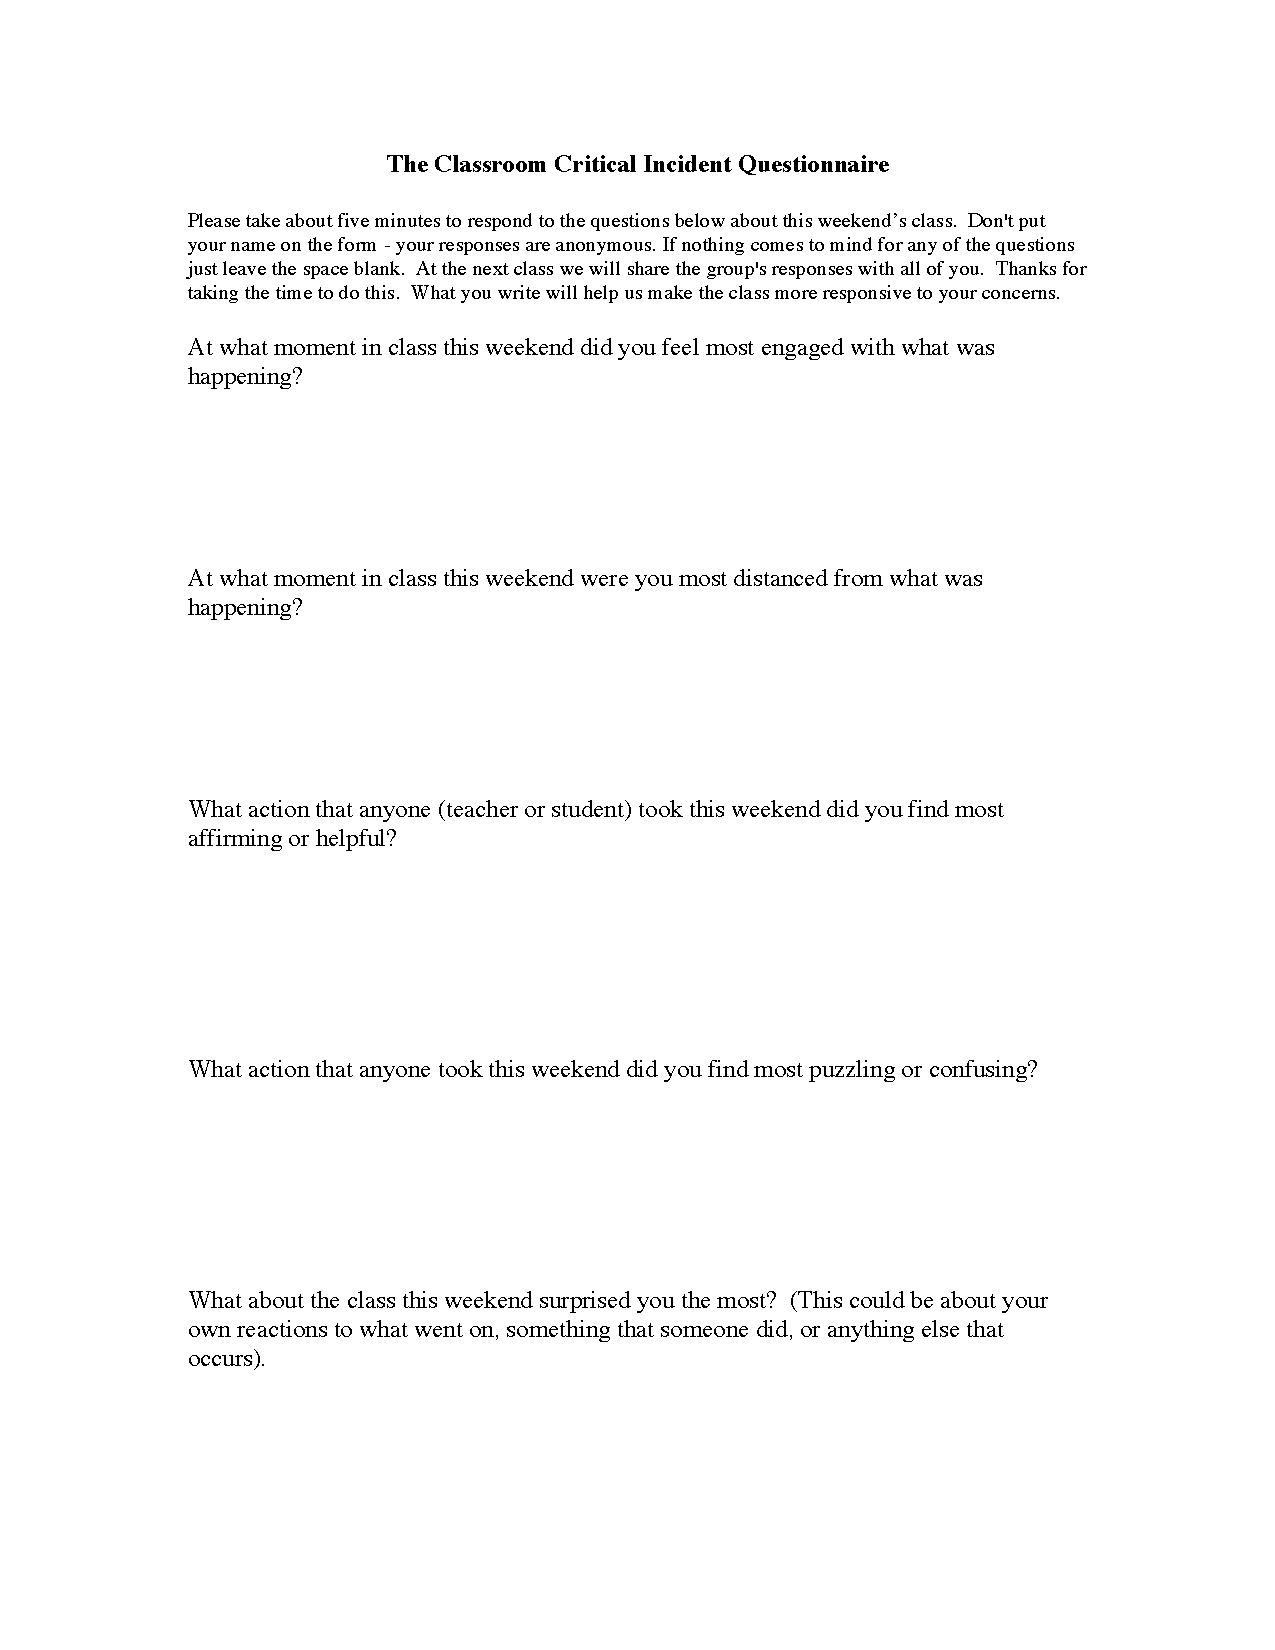
\includepdf[pages=-]{CIQ.pdf}
\subsection*{CIQ Summary of Student Responses}
\begin{center}
  \begin{tabular}{rp{4in}}
    \textbf{Question 1:}& At what moment in class this week did you feel most engaged with what was
happening?\\
        \textbf{Top Response:}& 
    \vspace{1 in}
    \\
    \textbf{Question 2:}& At what moment in class this week were you most distanced from what was
happening? \\
        \textbf{Top Response:}& 
    \vspace{1 in}
    \\
    \textbf{Question 3:}& What action that anyone (teacher or student) took this week did you find most
affirming or helpful \\
        \textbf{Top Response:}& 
    \vspace{1in}
    \\
    \textbf{Question 4:}& What action that anyone took this week did you find most puzzling or confusing?\\
        \textbf{Top Response:}& 
    \vspace{1 in}
    \\
     \textbf{Question 5:}&What about the class this week surprised you the most? (This could be about your own reactions to what went on, something that someone did, or anything else that
occurs).
\\
    \textbf{Top Response:}& 
    \vspace{1 in}
    \\
  \end{tabular}
\end{center}

\subsection*{Changes planned by Instructor}How will you (the instructor) make changes to accommodate the student feedback.  If choosing not to, explain. The best practice is to provide students with the summary of their responses (i.e. top replies) and indicate what changes you are implementing to address these.
\vspace{2.5 inches}

\subsection*{Instructor reflection on any changes made}

\vspace{2.5 inches}
}